\documentclass[12pt,a4paper]{article}
\usepackage[utf8]{inputenc}
\usepackage[T2A]{fontenc}  
\usepackage[russian]{babel}
\usepackage[margin=1cm]{geometry}
\usepackage{amsmath}
\usepackage{amsfonts}
\usepackage{amssymb}
\usepackage{graphicx}
\usepackage{float}
\usepackage{bm}

\begin{document}

\title{\textbf{Определение оптимальной толщины конвертера}}
\author{Эннс Сергей}
\date{\today}
\maketitle

Конвертер служит для преобразования фотонов в электрон-позитронные пары. 
Далее заряженные частицы фиксируются на детекторе, на основе этих данных проводится подгонка изначального распределения фотонов.
В области малых толщин эффективность подгонки быстро растёт, поскольку большее число фотонов участвует в рождении пар, что увеличивает количество регистрируемых событий. Однако при больших толщинах количество взаимодействующих фотонов выходит на плато и начинает доминировать многократное рассеяние электронов и другие электромагнитные процессы, приводящие к уширению пятна и постепенной потере информации о поляризации.

Зависимость эффективности подгонки поляризации 
\[
\frac{P^*}{\sigma_{P^*}}
\]
от толщины конвертера хорошо аппроксимируется асимметричной гауссианой — функцией, составленной из двух половин гауссовых кривых с различными значениями $\sigma$ слева и справа от максимума:
\[
f(x) = A \cdot \exp\left(-\frac{(x-x_0)^2}{2\sigma^2(x)}\right) + c,
\]
где $\sigma(x) = \sigma_{\text{left}}$ при $x < x_0$ и $\sigma(x) = \sigma_{\text{right}}$ при $x \ge x_0$.

Параметр $x_0$ определяет оптимальную толщину конвертера, при которой достигается максимальная эффективность подгонки.

Результаты аппроксимации для вольфрама представлены на рис.\ref{fig:wolphram}. Оптимальная толщина составила $x_0 = 8.00 \pm 0.34$ мм.

\begin{figure}[H]
    \centering
    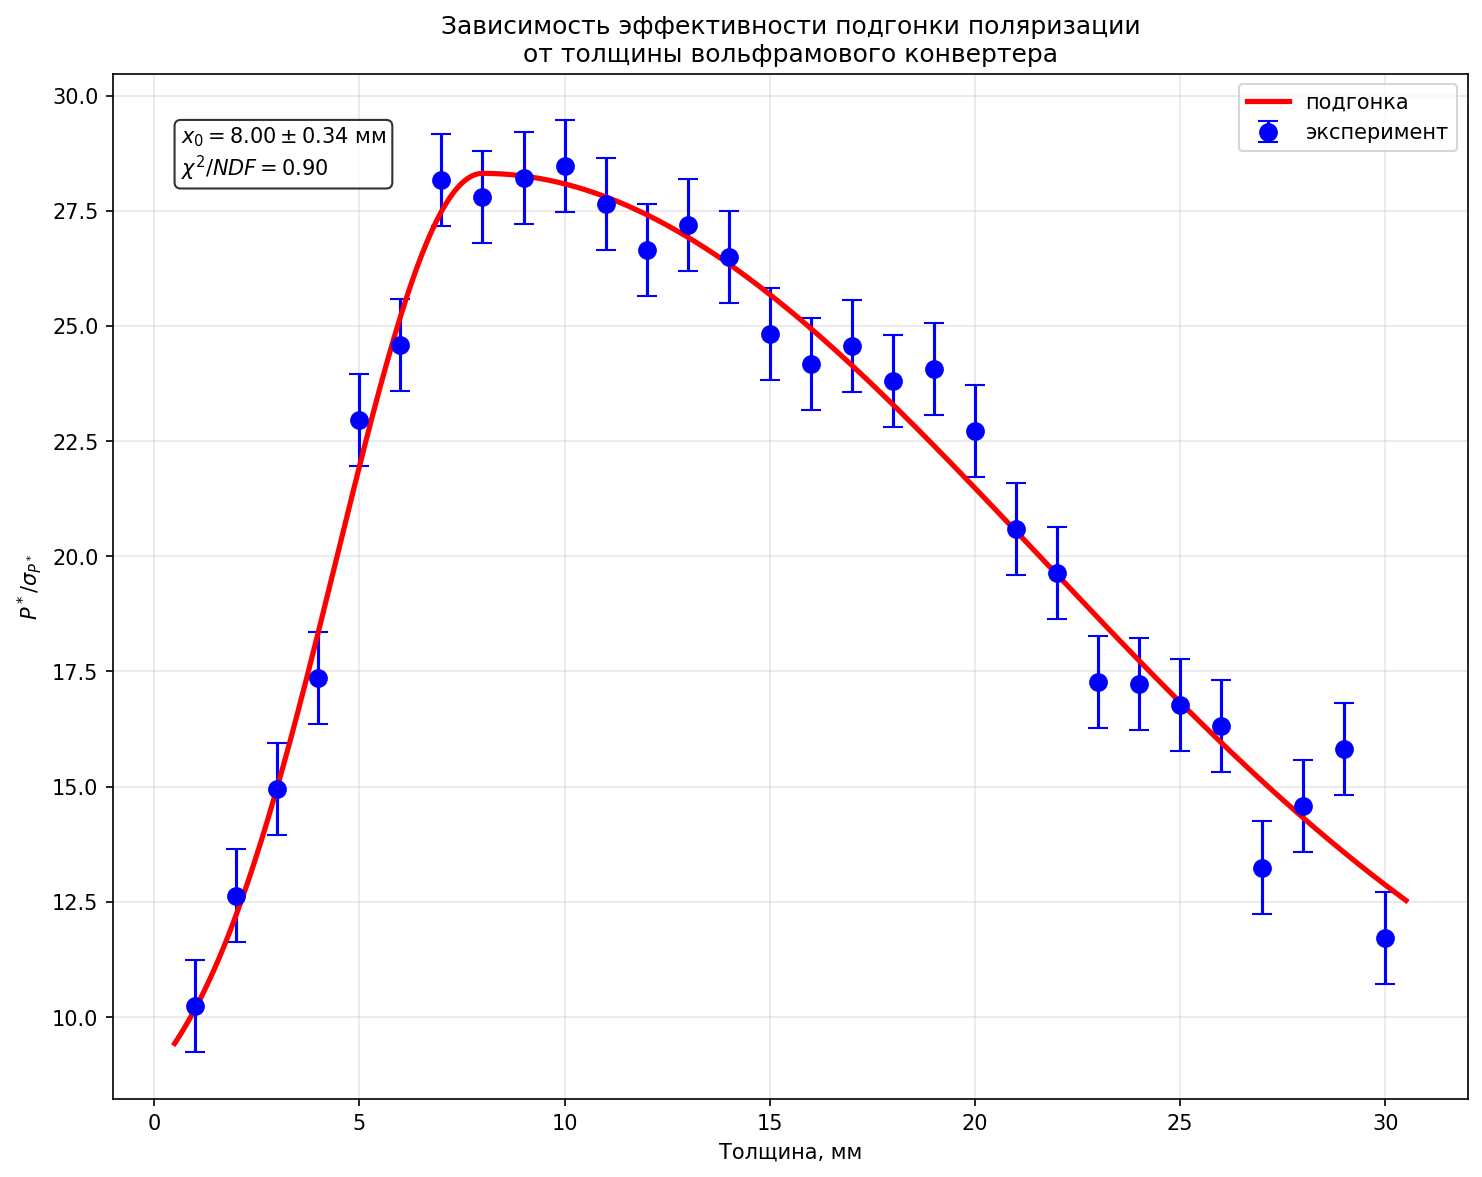
\includegraphics[width=0.7\linewidth]{wolphram.png}
    \caption{Зависимость эффективности подгонки поляризации от толщины вольфрамового конвертера}
    \label{fig:wolphram}
\end{figure}

Для сравнения аналогичная процедура была выполнена для свинца (рис.~\ref{fig:plumbum}).

\begin{figure}[H]
    \centering
    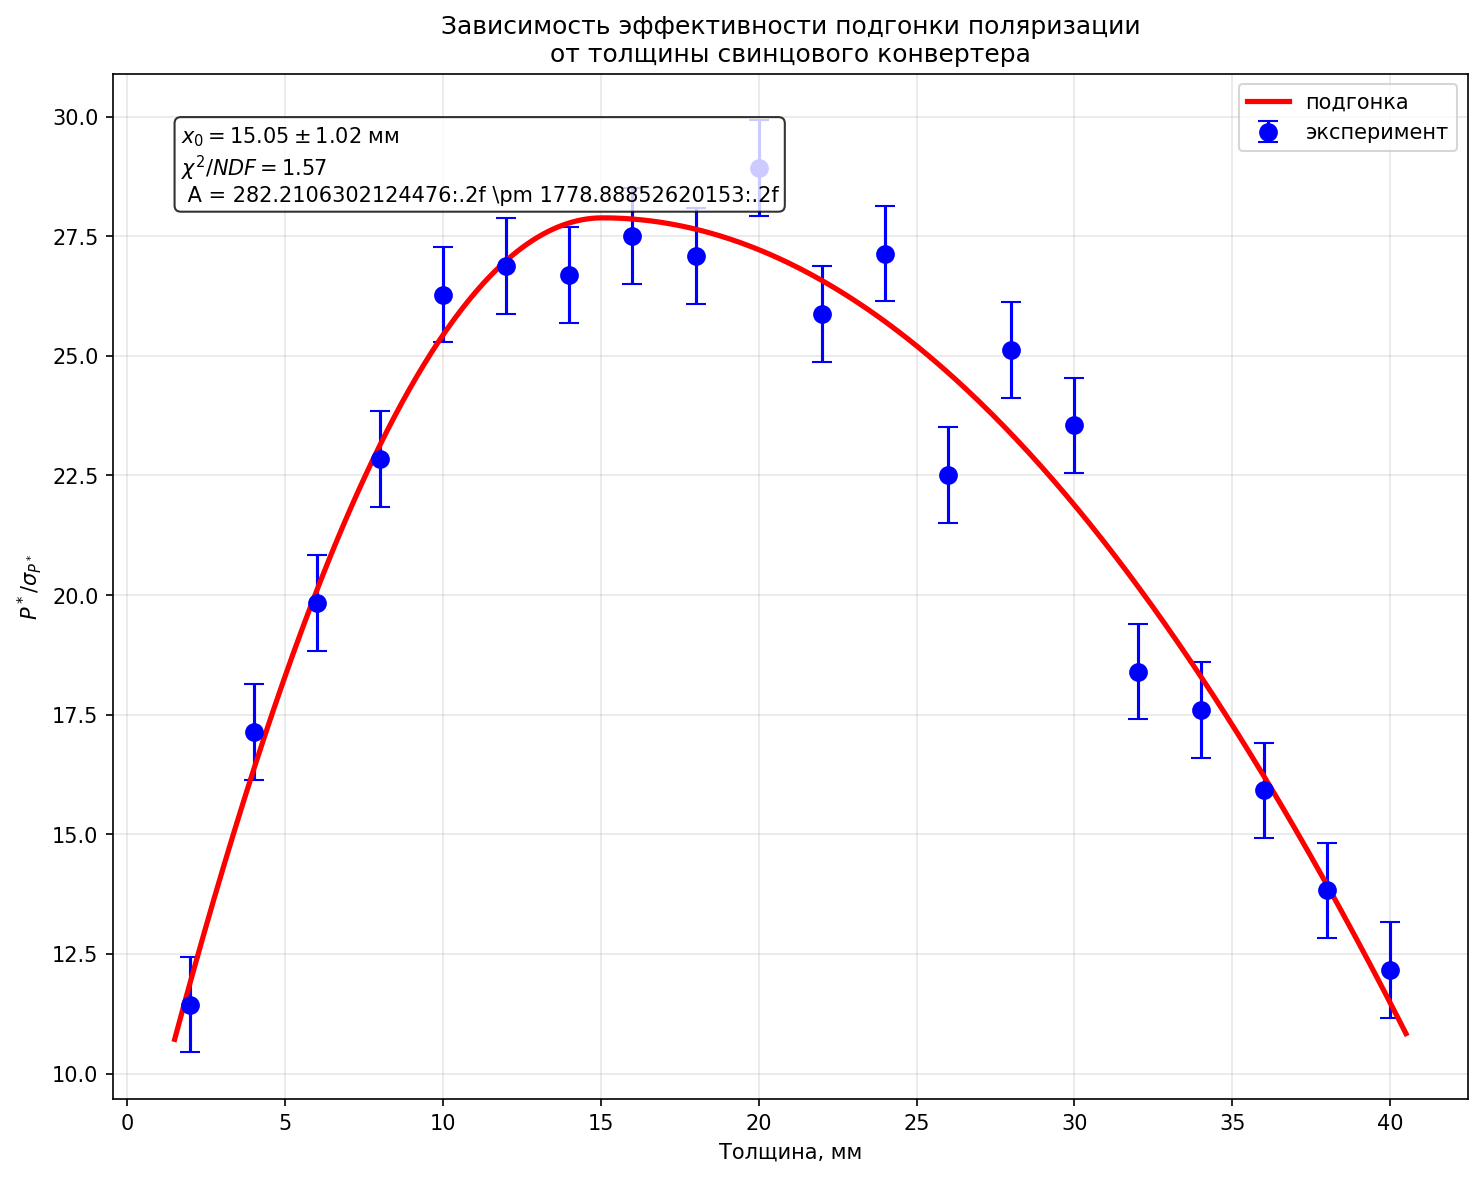
\includegraphics[width=0.7\linewidth]{plumbum.png}
    \caption{Зависимость эффективности подгонки поляризации от толщины свинцового конвертера}
    \label{fig:plumbum}
\end{figure}

Как видно из полученных результатов, вольфрам имеет меньшую оптимальную толщину по сравнению со свинцом, что позволяет экономить материал конвертера при сохранении высокой эффективности подгонки поляризации.

\end{document}